\section{Incarnation 1}
  \begin{flushleft}
    The logic for computing Cos, Sin, Pi and other functions were written from the ground up in this incarnation. See snippets below.
  \end{flushleft}
  \subsection{Snippets}
  \vspace{2em}
    \begin{figure}[h!]
      \centering
      \frame{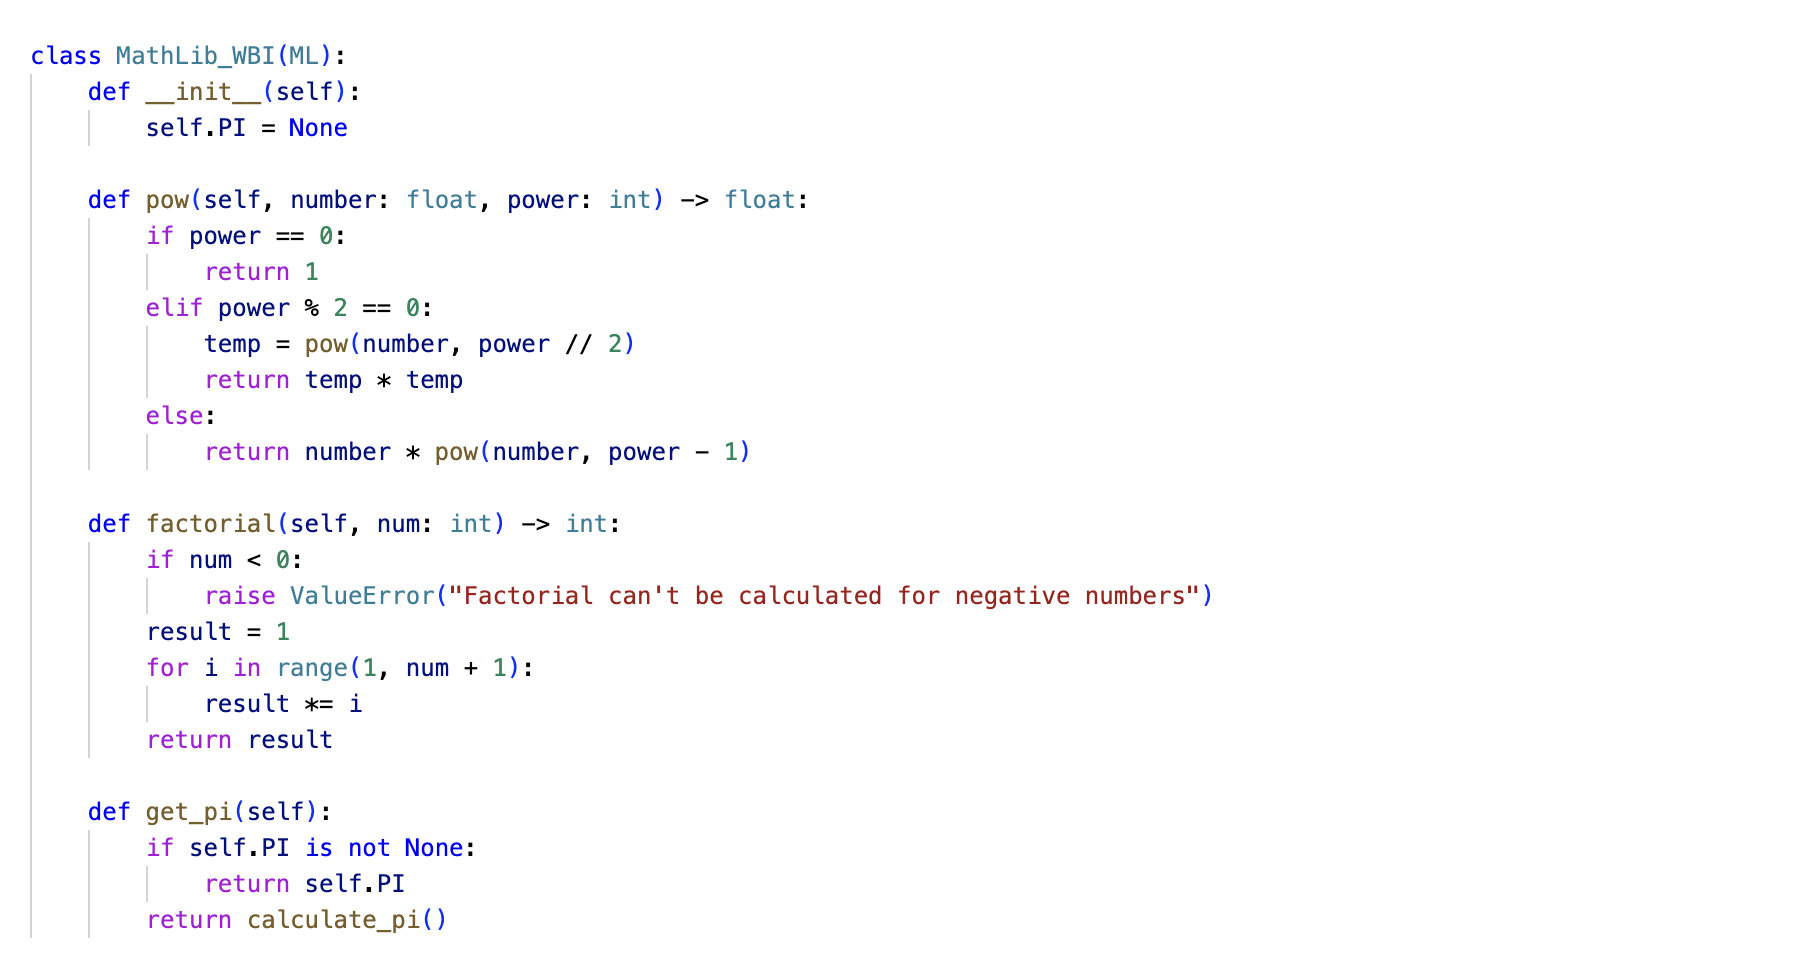
\includegraphics[scale= 0.4]{resources/snippets/MathWBI.png}}
      \caption{Logic to compute Exponent, Factorial and Pi}
      \label{fig:Math Library}
    \end{figure}
    \pagebreak
    \begin{figure}[h!]
      \centering
      \frame{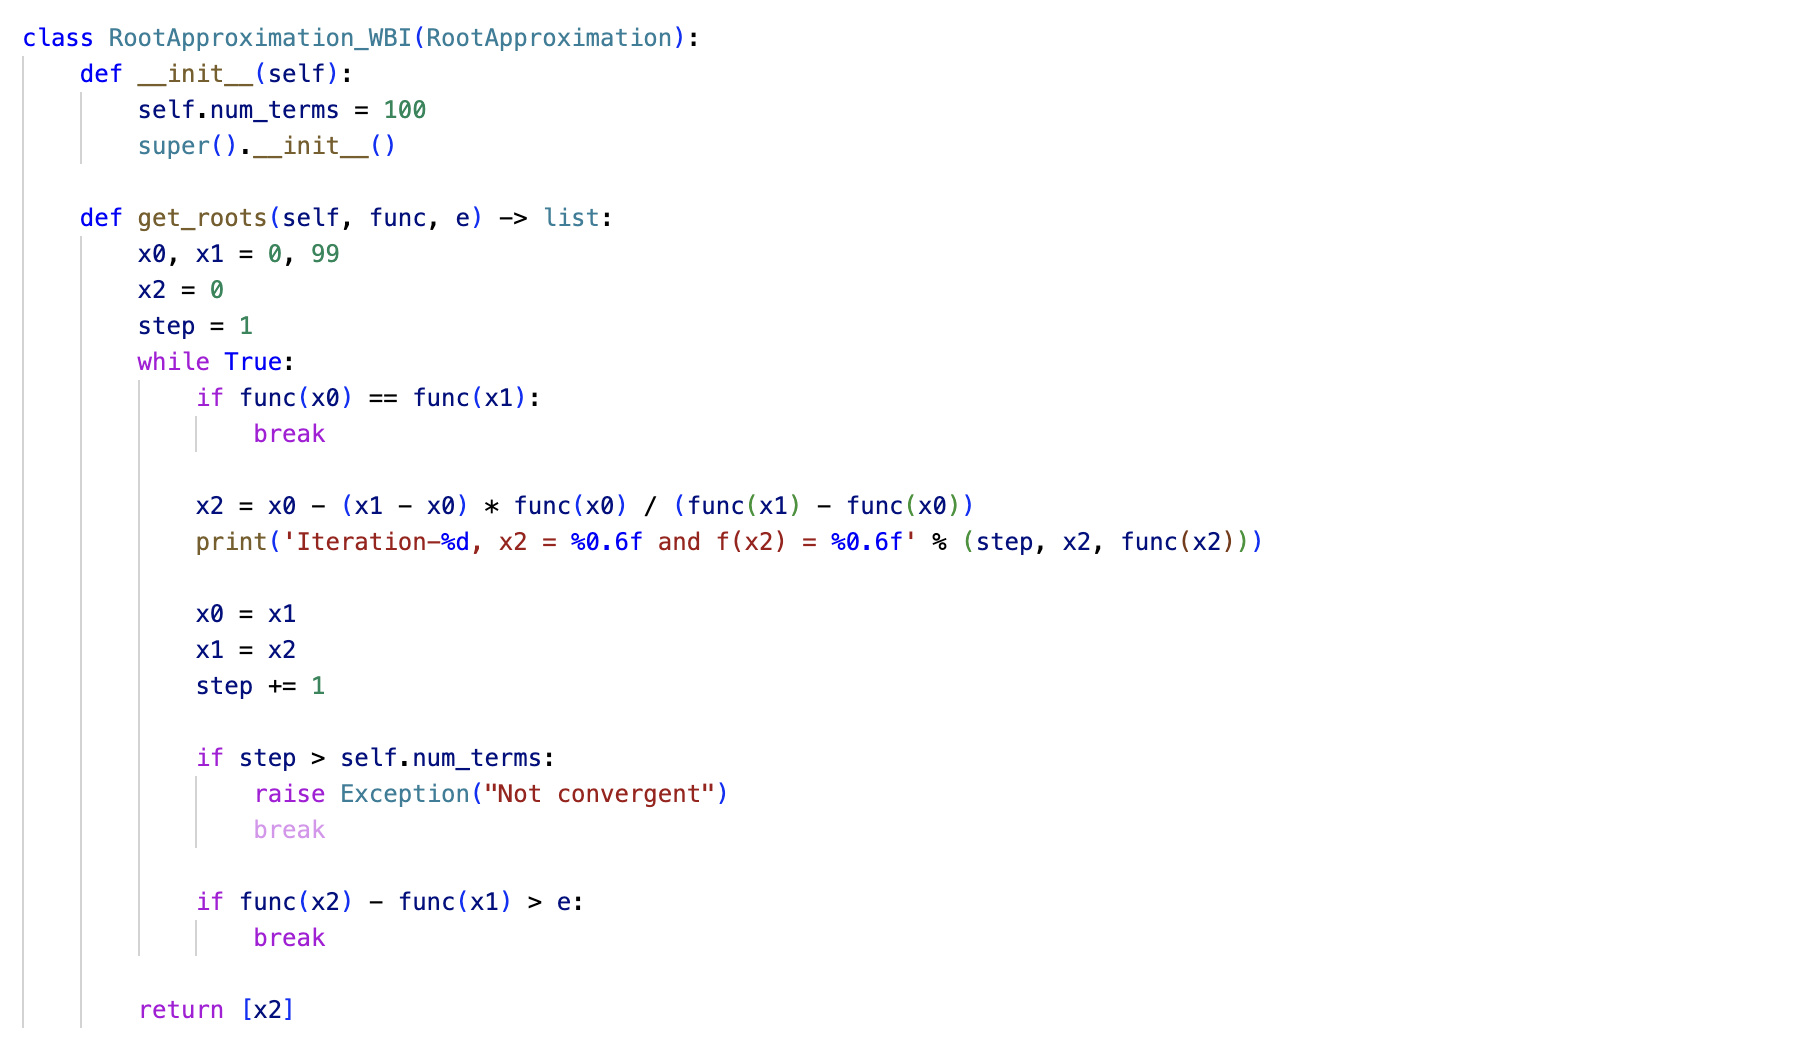
\includegraphics[scale= 0.4]{resources/snippets/RootApWBI.png}}
      \caption{Secant Method of root approximation}
      \label{fig:Root Approximation}
    \end{figure}

    \begin{figure}[h!]
      \centering
      \frame{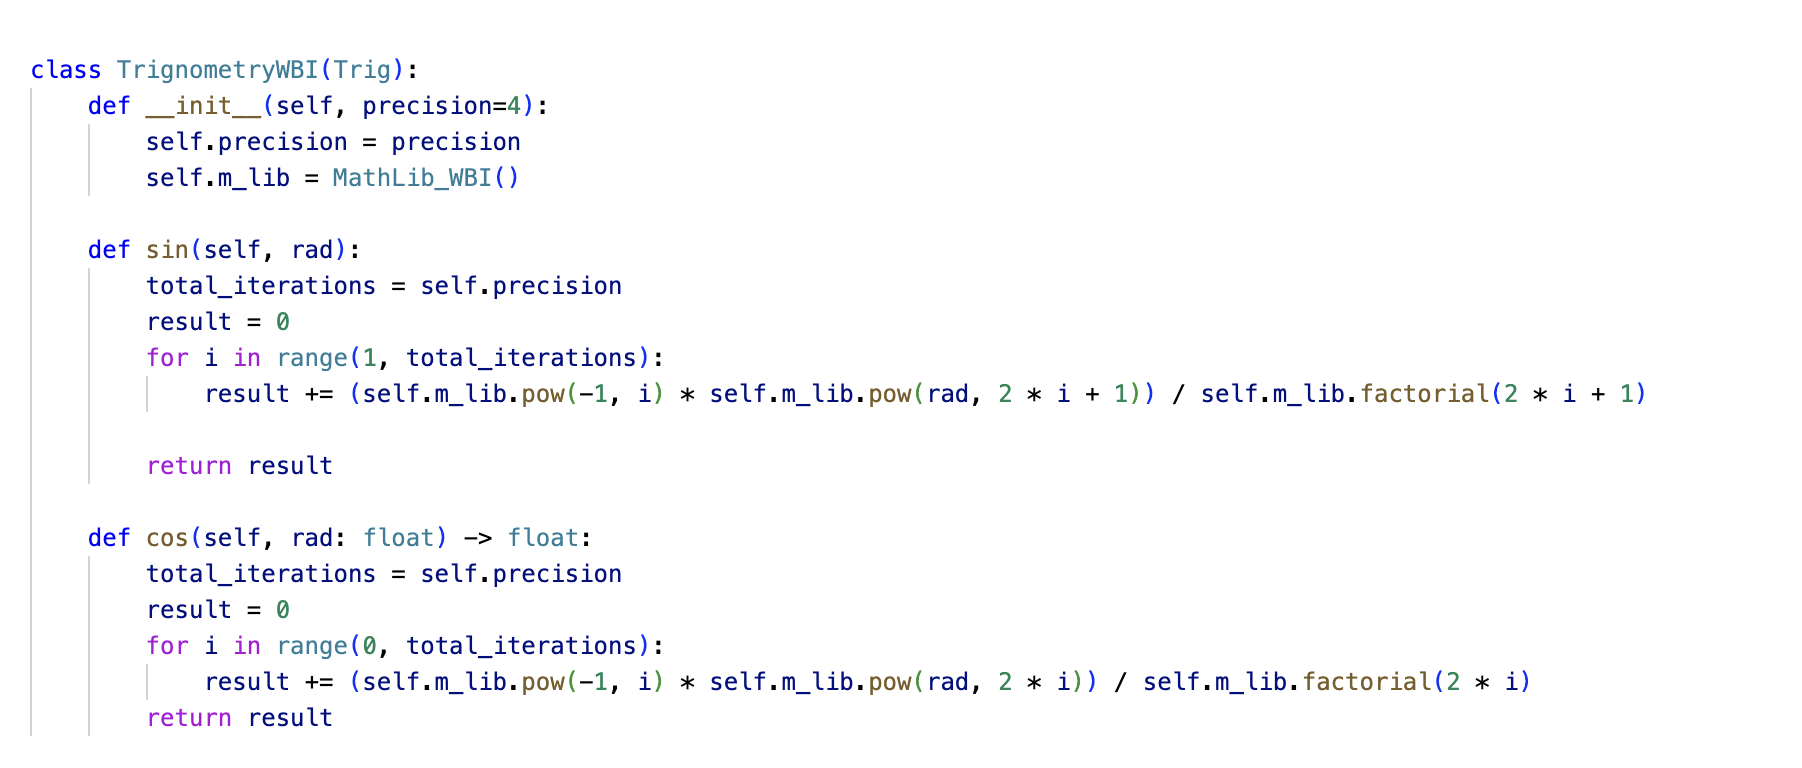
\includegraphics[scale= 0.4]{resources/snippets/TrigonometryWBI.png}}
      \caption{Logic to compute trigonometry functions}
      \label{fig:trigonometric Functions}
    \end{figure}
    \pagebreak

    \subsection{Output}
    \begin{figure}[h!]
      \centering
      \frame{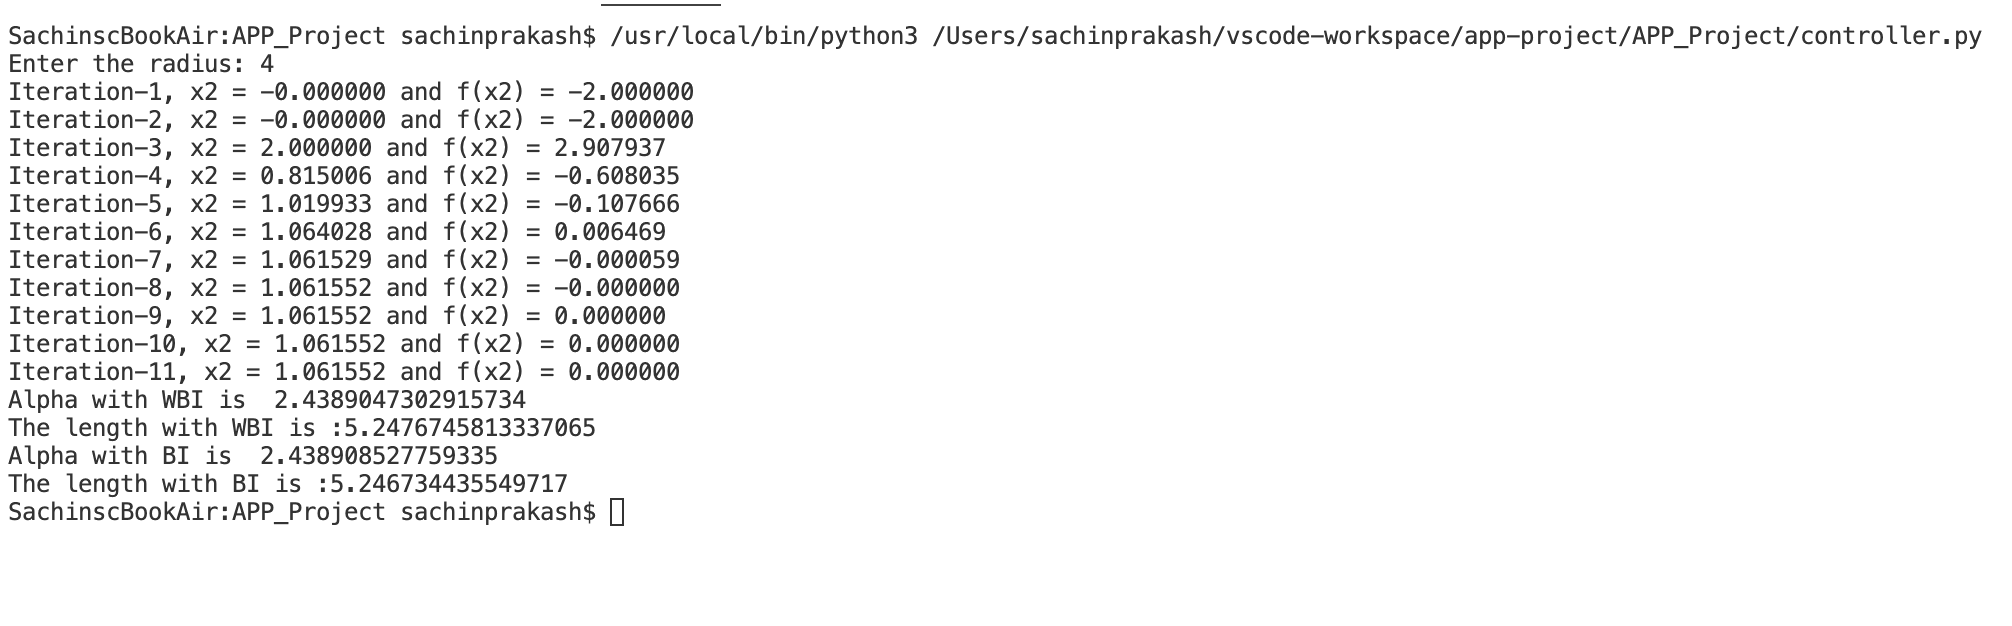
\includegraphics[scale= 0.4]{resources/snippets/inc1OP.png}}
      \caption{Output for Incarnation 1}
      \label{fig:Text-based output}
    \end{figure}
    \pagebreak

\section{Incarnation 2}
  \begin{flushleft}
    The python Math module and SciPy library was used to compute the various values. See snippets below.
  \end{flushleft}

  \subsection{Snippets}
  \vspace{2em}
    \begin{figure}[h!]
      \centering
      \frame{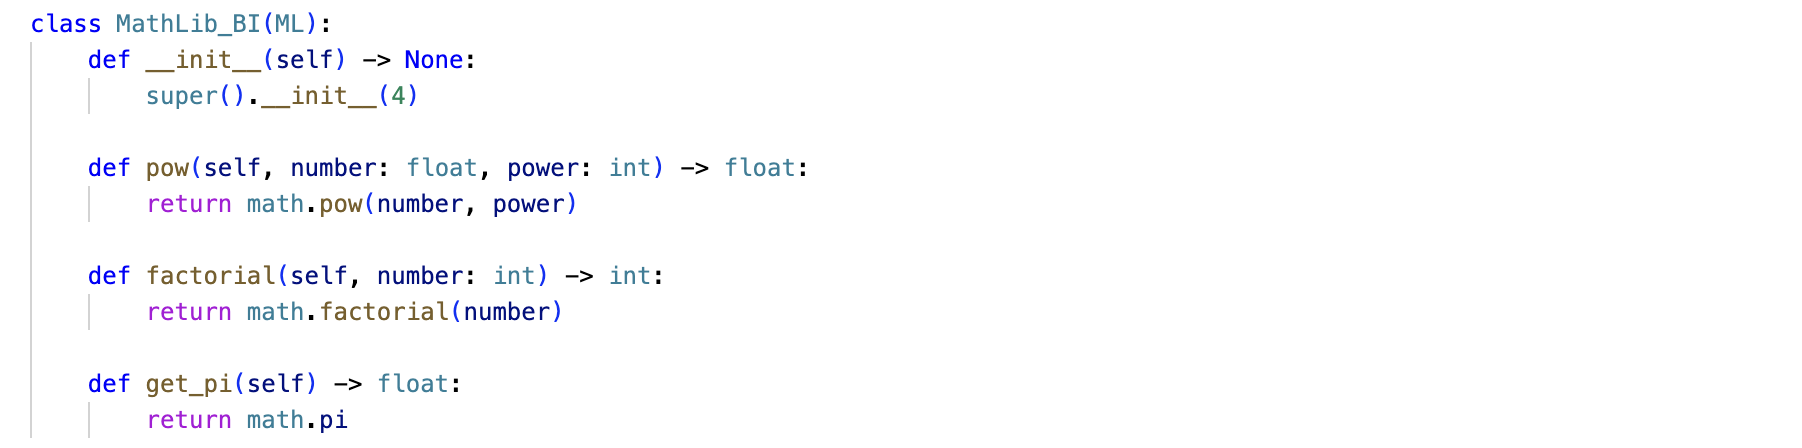
\includegraphics[scale= 0.4]{resources/snippets/MathBI.png}}
      \caption{Math module functions}
      \label{fig:Library functions for math}
    \end{figure}

    \begin{figure}[h!]
      \centering
      \frame{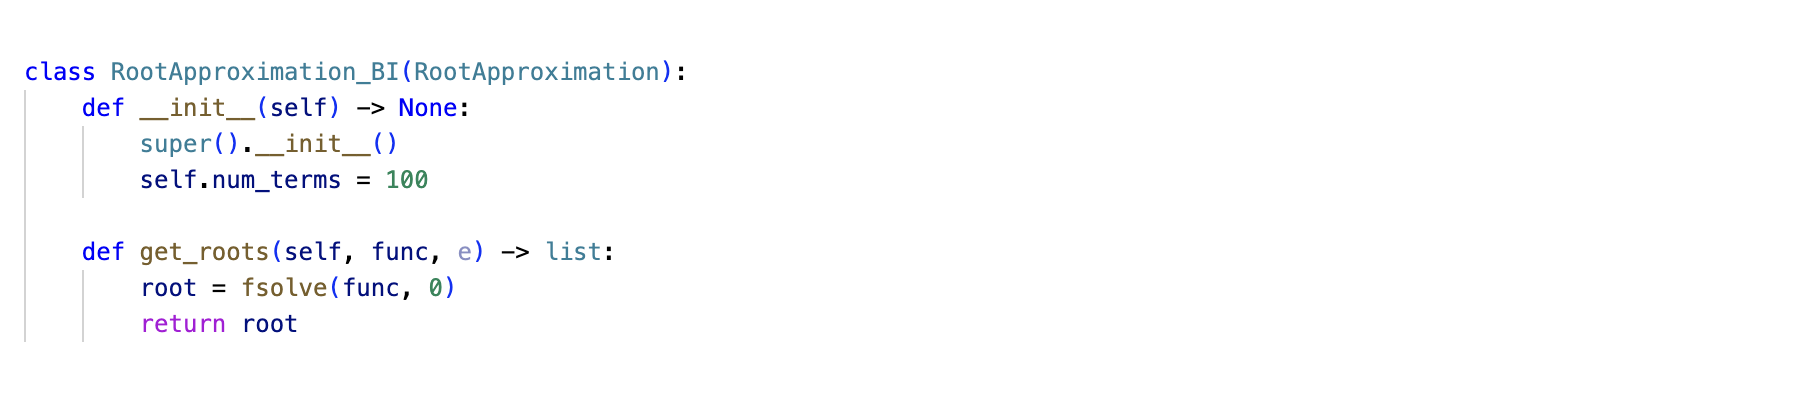
\includegraphics[scale= 0.4]{resources/snippets/RootApBI.png}}
      \caption{Root approximation using SciPy}
      \label{fig:SciPy Root Approximation}
    \end{figure}

    \begin{figure}[h!]
      \centering
      \frame{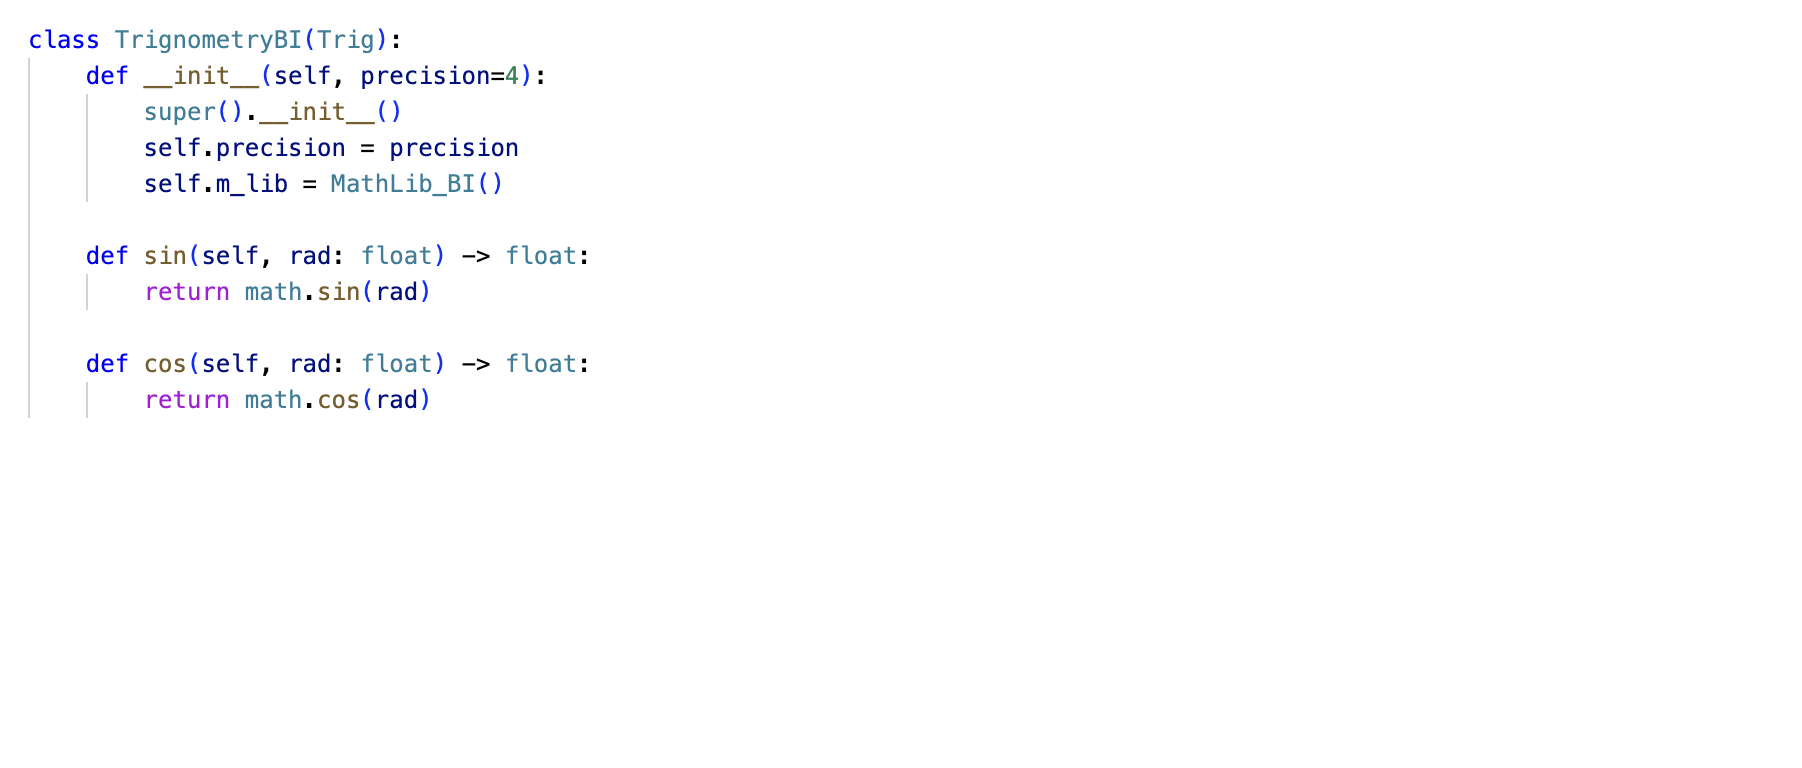
\includegraphics[scale= 0.4]{resources/snippets/TrigonometryBI.png}}
      \caption{Math module Trigonometry functions}
      \label{fig:Math trigonometry functions}
    \end{figure}
    \pagebreak

    \subsection{Output}
    \begin{figure}[h!]
      \centering
      \frame{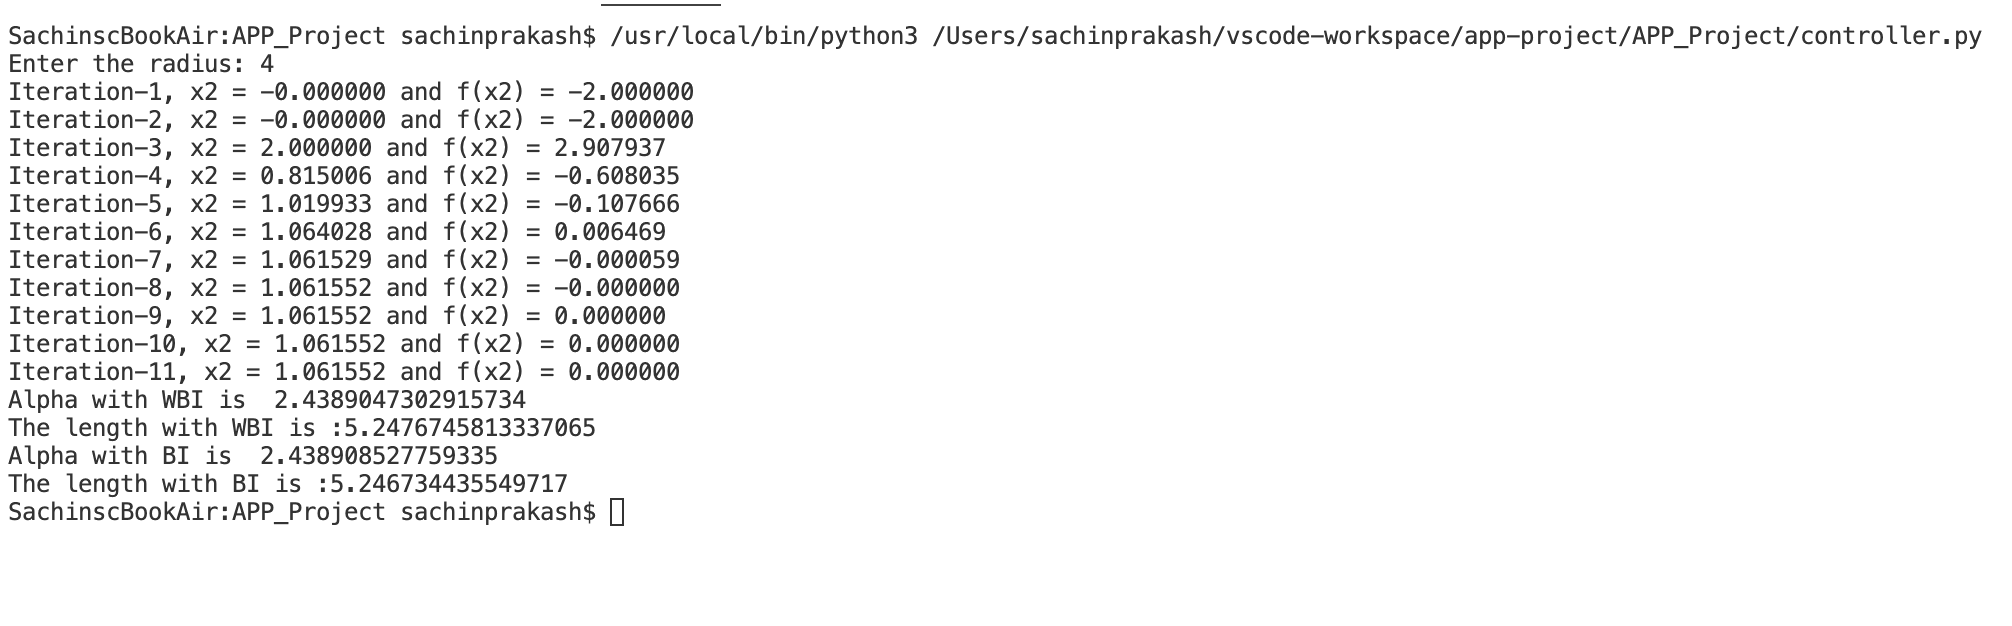
\includegraphics[scale= 0.4]{resources/snippets/inc1OP.png}}
      \caption{Update this - include XML DTD}
      \label{fig:XML output}
    \end{figure}

\section{Quality Attributes}
  \begin{flushleft}
    The following attributes are applicable to both incarnations.
  \end{flushleft}
  \hiddensubsection{Modifiability}
    \begin{flushleft}
      Modifiability refers to flexibility of a system to incorporate changes. The source code was built using the RDD paradigm. This inherently makes it amenable to updates in the future.
    \end{flushleft}

  \hiddensubsection{Readability}
    \begin{flushleft}
      Adequate comments were provided to make the source code more meaningful to the reader. The variable and method names adhere to the guidelines provided under PEP 8. 
    \end{flushleft}

  \hiddensubsection{Resuability}
    \begin{flushleft}
      The source code was made reuseable by following the Single Responsibility Principle (SRP) for every class and method. Abstract types have been used to hide the implementation details and improve the composability.
    \end{flushleft}

  \hiddensubsection{Understandability}
    \begin{flushleft}
      The understandability of the source code was improved through
      \begin{itemize}
        \item {The use of meaningful variable names}
        \item {Inclusion of method and class descriptions}
        \item {Minimizing the complexity within each method in a class}
      \end{itemize}
    \end{flushleft}

  \hiddensubsection{Testability}
    \begin{flushleft}
      Due to the object-oriented nature of the project design, each class and method in the source code can be unit tested. Each class has it's own set of tests which can swiftly determine if the actual value matches the expected.
    \end{flushleft}

  \hiddensubsection{Robustness}
  \begin{flushleft}
    All possible exceptions have been handled throughtout the program and the potential points of failure have been minimized. In case of an exceptional event, a meaningful error message will be returned to the end user.
  \end{flushleft}

  \hiddensubsection{Generality}
    \begin{flushleft}
      The program has been made more general by avoiding the use of OS specific path(s). Eg: When writing to an output file, relative path name was used.
    \end{flushleft}

    \hiddensubsection{Usability}
    \begin{flushleft}
      The usability of the program has been improved by 
      \begin{itemize}
        \item {Using meaningful prompt messages throughtout the lifecycle }
        \item {Minimizing the potential points of failure }
        \item {Returning meaningful error messages in case of an exceptional event}
      \end{itemize}
    \end{flushleft}

